\chapter{Numerical boundary conditions for SPM concentrations}
\pagenumbering{roman}

In view of the strong near-bottom gradients of suspended material, the
implementation of the boundary conditions for the SPM transport
equation \eq{c} requires special attention. While \eq{defFz} provides
an exact expression for the upward turbulent flux $F_z$ at the bottom,
the numerical implementation of the sinking flux,
\begin{equation}
 \label{Fs}
 F_s(z=0) = w_s c_0 \comma
\end{equation}
is not straightforward because the bottom concentration, $c_0$, is
unknown. In vertically staggered numerical grids typically used in
ocean modeling, the bottom concentration $c_0$ has to be estimated
from the known concentration $c_1$ in the center of the lowermost grid
cell, which requires some assumptions about the vertical distribution
of the suspended material in the near-bottom region. While it is
reasonable to assume that the bottom cell is well mixed (i.e.,
$c_0=c_1$) if the bed stress $|\tau_b|$ is smaller than the critical
stress for erosion, $\tau_c$, it is likely that the bottom
concentration $c_0$ is significantly larger than $c_1$ if active
erosion takes place ($|\tau_b| > \tau_c$). In this case, the popular
assumption $c_0=c_1$ may lead to large numerical errors, and to a grid
dependence of the numerical solution. In the following, we show how a
more consistent lower boundary condition can be derived.

We start from the observation that close to the bottom, the transport
equation in \eq{c} reduces to a balance between upward mixing and
downward sinking of suspended material,
\begin{equation}
 \label{cstationary}
 0 = \nu_t^b \partder{c}{z} + w_s c
 \comma
\end{equation}
assuming small slopes ($\alpha \ll 1$) for simplicity. The turbulent
viscosity in the near-bottom region is known to follow the
law-of-the-wall relation $\nu_t = \kappa u_\ast (z + z_0)$, where
$\kappa \approx 0.4$ is the von K{\'a}rm{\'a}n constant, and $u_\ast =
|\tau_b|^{1/2}$ the bottom friction velocity
\citep[e.g.,][]{Pope2000a}. The turbulent diffusivity $\nu_t^b$ in this
region is proportional to $\nu_t$, and therefore adopts the form
$\nu_t^b = Pr_t^{-1} \kappa u_\ast (z + z_0)$, where the turbulent
Prandtl number, $Pr_t$, plays the role of a constant proportionality
factor of order 1. The turbulence model used in our study has been shown to
exactly reproduce this near-wall behavior for $\nu_t$ and $\nu_t^b$
\citep[e.g., ][]{UmlaufBurchard2003a,UmlaufBurchard2005a}.

Inserting the above law-of-the-wall relation for $\nu_t^b$ into
\eq{cstationary}, we find a solution of the form
\begin{equation}
 \label{Rouse}
 \dfrac{c}{c_0} = \left( \frac{z}{z_0} + 1 \right)^{-p} \comma
\end{equation}
which is recognized as the classical Rouse profile
\citep{vanRijn84b}, slightly modified here by the appearance of the
turbulent Prandtl number in the definition of the Rouse number $p =
w_sPr_t \, / (\kappa u_\ast)$.

Recalling that in any conservative numerical scheme, $c_1$ represents
the average concentration inside the lowermost grid cell, a relation
between $c_0$ and $c_1$ may be found from integrating \eq{Rouse}
across the cell. If we denote $h$ as the cell thickness, this yields
\begin{equation}
 \label{cbot}
 c_0 = \frac{c_1}{r} \quad \text{for} \quad |\tau_b|>\tau_c \comma
\end{equation}
where 
\begin{equation}
 \label{rr}
 r =  \frac{1}{(1-p) h/z_0} \left[ \left( \frac{h}{z_0} + 1 \right)^{1-p} -1 \right] 
 \comma
\end{equation}
\begin{figure}[h]
  \noindent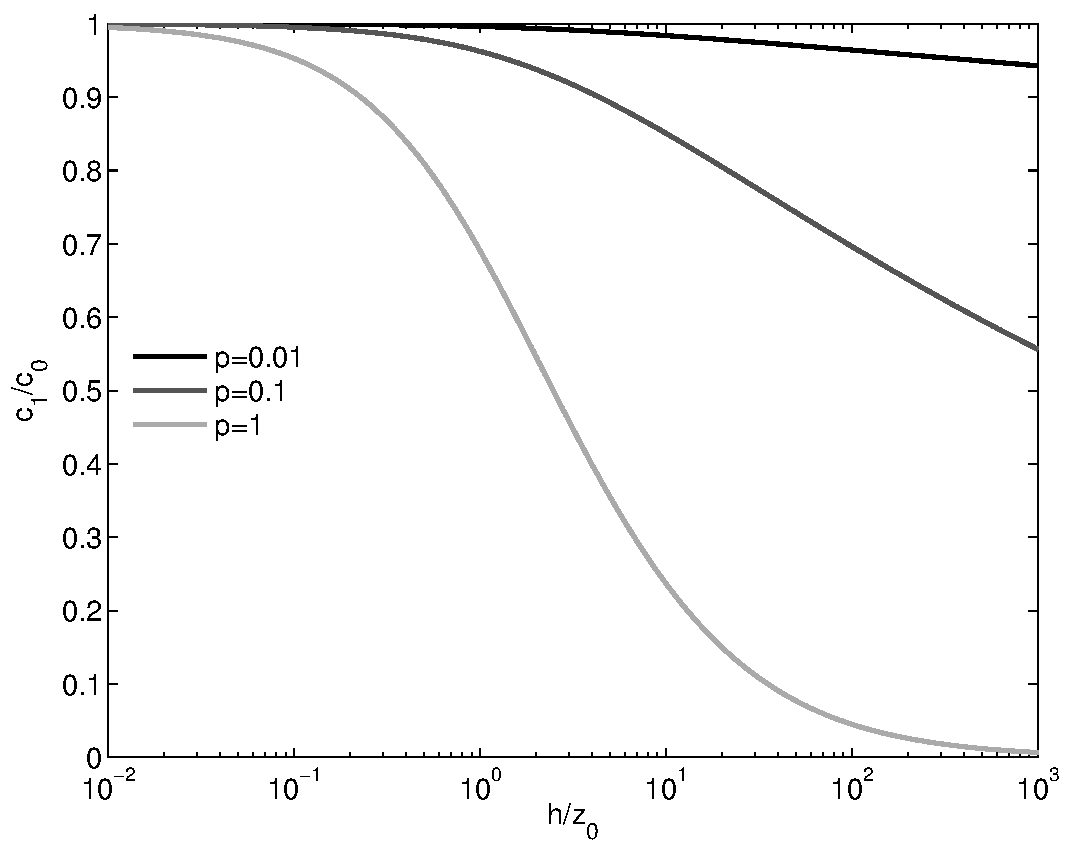
\includegraphics[width=29pc,angle=0]{bilder/rouse.pdf}\\
  \caption{A1}{Concentration ratio $c_1/c_0$ as a function of
    non-dimensional cell thickness, $h/z_0$, for different Rouse
    numbers according to \eq{cbot}.\label{c0c1}}
\end{figure}
Fig. A1 shows the ratio $r=c_1/c_0$ as a function of the normalized
cell thickness $h/z_0$ for different Rouse numbers. The most important
conclusion from this figure is that the naive approach of assuming
$c_0 = c_1$ to compute the sinking flux in \eq{Fs} during erosion
periods introduces large numerical errors except for small Rouse
numbers and/or extremely fine grids with $h \ll z_0$. Below, we
nevertheless discuss some reference solutions that satisfy this
condition. We note, however, that the constraint $h \ll z_0$ implies
$\Delta t \ll z_0 / w_s$ for the numerical time step according to the
well-known CFL stability criterion for explicit advection schemes. It
is easy to show that, even for idealized one-dimensional simulations,
the numerical effort may become prohibitively large for small $z_0$.

Using the example from Section \ref{sec:bbl} above, Fig. A2
illustrates that assuming $c_0 = c_1$ during both erosive and
non-erosive periods leads to significant numerical errors, and to a
grid-dependence of the results. 
\begin{figure}[h]
  \noindent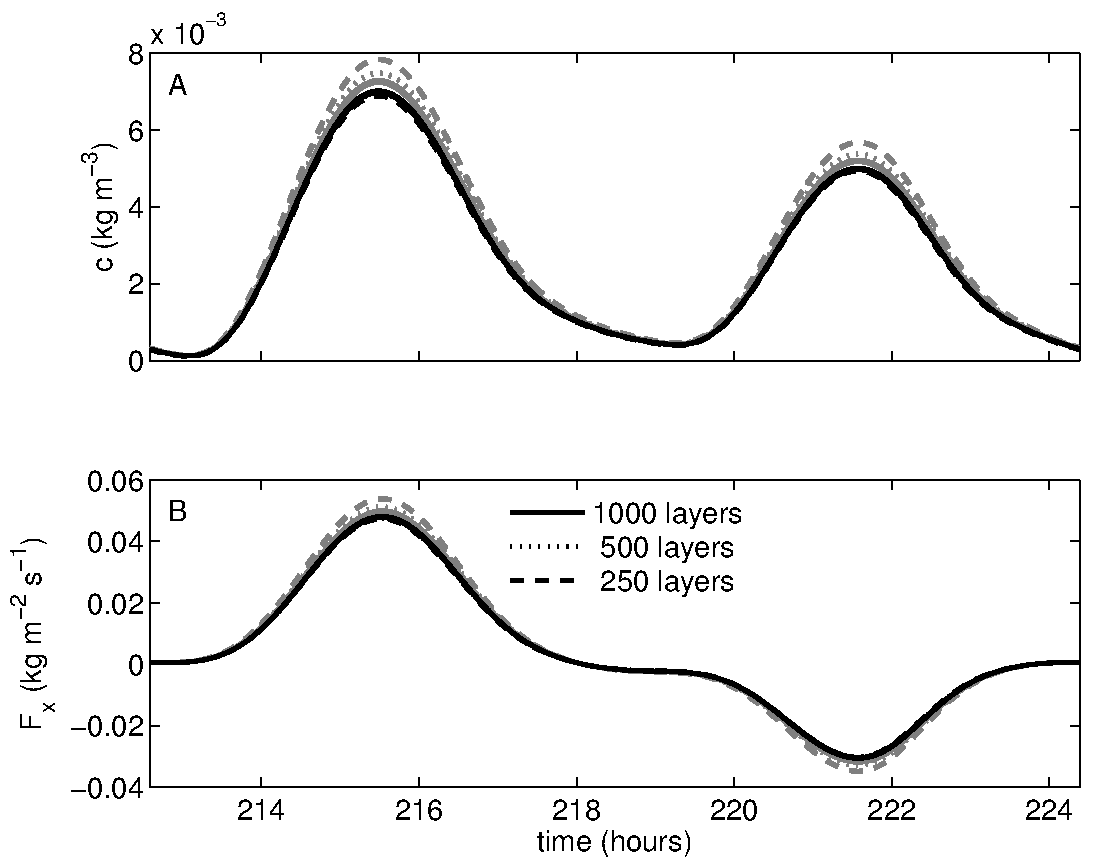
\includegraphics[width=29pc,angle=0]{bilder/appendix.pdf}\\ \caption{A2}{Numerical
    results for (a) SPM concentration 5~m above the bottom, and (b)
    upslope flux $F_x$ for three vertical resolutions. Gray lines are
    based on the assumption $c_0 = c_1$ to compute the sinking flux in
    \eq{Fs}, whereas black lines are based on \eq{cbot} during erosive
    periods. Parameters correspond to Case 1 in
    \tab{params}. \label{convergence}}
\end{figure}
Estimating $c_0$ based on \eq{cbot}
during periods with active erosion, however, removes this dependency
on the numerical grid, and leads to stable results already for
moderate vertical resolution. All results discussed in this manuscript
are therefore based on this new expression. Convergence studies were
carried out to insure that all our results are independent of the
numerical grid size and time step.